\documentclass[12pt]{report}
\usepackage[dvipdfmx]{graphicx}
\usepackage[color]{coqdoc}
\usepackage[bookmarks=false,dvipdfmx,hidelinks,setpagesize=false]{hyperref}
\usepackage[all]{xy}
% ``xy''については
% http://www.math.sci.hokudai.ac.jp/~abenori/tex/index.html#xy-pic を参照

\usepackage[utf8x]{inputenc}
\usepackage{tipa}

\usepackage[T1]{fontenc}
\usepackage{fullpage}
\usepackage{amsmath,amssymb,url,ascmac,fancyhdr}


\newcommand{\HRule}{\rule{\linewidth}{0.5mm}}
\newcommand{\domain}[1]{\lfloor #1 \rfloor}

\newtheorem{definition}{\bf Definition}
\newtheorem{theorem}{\bf Theorem}
\newtheorem{example}{\bf Example}
\newtheorem{lemma}{\bf Lemma}
\newtheorem{axiom}{\bf Axiom}
% \newenvironment{code}{\footnotesize\lstlisting}{\endverbatim\normalsize}
\newcommand{\rel}{\rightharpoondown}
\newcommand{\id}{\mbox{id}}

\begin{document}

% \title{Coq Modules for Relational Calculus (Ver.0.2)}
% \author{Hisaharu Tanaka \and Shuichi Inokuchi \and Yoshihiro Mizoguchi
% \and Toshiaki Matsushima}
% \date{\today}
% \maketitle

\begin{titlepage}
\begin{center}
% Upper part of the page. The '~' is needed because \\
% only works if a paragraph has started.
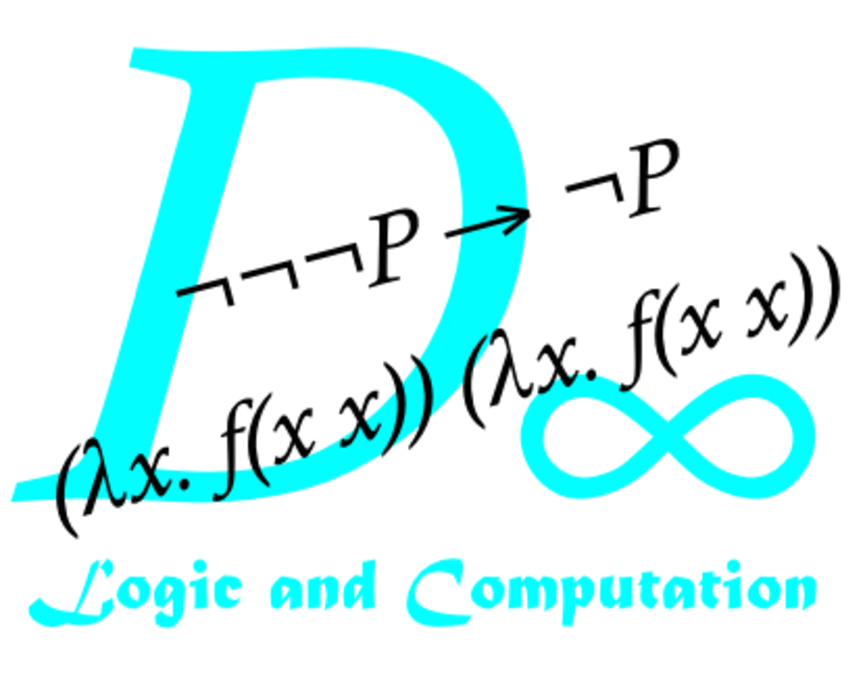
\includegraphics[width=0.35\textwidth]{./TPPLOGO.pdf}~\\[2cm]

\textsc{\Large Institute of Mathematics for Industry,} \\
\textsc{Kyushu University}\\[1.5cm]

\textsc{\Large Logic and Computation Project}\\[0.5cm]

% Title
\HRule \\[0.4cm]
{ \huge \bfseries Coq Modules for Relational Calculus }\\[0.2cm]
(Ver.0.1)\\[0.4cm]

\HRule \\[1.5cm]

% Author and supervisor
\begin{center}
\begin{minipage}[t]{0.4\textwidth}
\begin{center} 
{\large Hisaharu \textsc{Tanaka}} \\
Saga University
\end{center}
\end{minipage}
\hspace{1cm}
\begin{minipage}[t]{0.4\textwidth}
\begin{center} 
{\large Toshiaki \textsc{Matsushima}} \\
Kyushu University
\end{center}
\end{minipage}
\end{center}
\begin{center}
\begin{minipage}[t]{0.4\textwidth}
\begin{center}
{\large Shuichi \textsc{Inokuchi}} \\
Fukuoka Institute of Technology
\end{center}
\end{minipage}
\hspace{1cm}
\begin{minipage}[t]{0.4\textwidth}
\begin{center} 
{\large Yoshihiro \textsc{Mizoguchi}} \\
Kyushu University
\end{center}
\end{minipage}
\end{center}
\vfill

% Bottom of the page
{\large \today}\\[1cm]
{\footnotesize
{\bf Repository:\ }
\url{https://github.com/KyushuUniversityMathematics/RelationalCalculus}}
\end{center}
\end{titlepage}

\tableofcontents

\setlength{\headheight}{15pt}
\colorlet{DEFGREEN}{black}
\pagestyle{fancy}
\fancyhead{}
\fancyhead[RE]{\rightmark}
\fancyhead[LO]{\leftmark}

\input{Basic_Notations.tex}
\input{Basic_Notations_Set.tex}
\input{Basic_Lemmas.tex}
\input{Relation_Properties.tex}
\input{Functions_Mappings.tex}
\input{Tactics.tex}
\input{Dedekind.tex}
\input{Conjugate.tex}
\input{Domain.tex}
\input{Residual.tex}
\input{Schroder.tex}
\input{Sum_Product.tex}
\input{Point_Axiom.tex}


\begin{thebibliography}{99}
\bibitem{affeldt2012}R. Affeldt and M. Hagiwara. Formalization of Shannon’s Theorems in SSReflect-Coq. In 3rd Conference on Interactive Theorem Proving, LNCS 7406, 233--249, 2012.
\end{thebibliography}

\end{document}
